\documentclass[tikz,border=12pt]{standalone}
\usepackage{amsmath,amssymb}
\usetikzlibrary{calc,arrows.meta}

\begin{document}
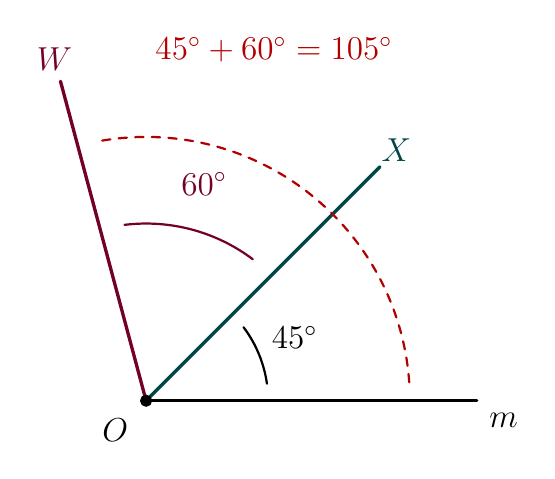
\begin{tikzpicture}[>=latex, line cap=round, line join=round]

  \coordinate (O) at (0,0);
  \def\R{4.2}

  % rays: Om at 0 deg, X at 45 deg, W at 105 deg
  \draw[very thick] (O) -- (\R,0);
  \draw[very thick, teal!55!black] (O) -- ($(O) + (45:\R)$) node[pos=1.07, font=\large\bfseries] {$X$};
  \draw[very thick, purple!60!black] (O) -- ($(O) + (105:\R)$) node[pos=1.07, font=\large\bfseries] {$W$};
  \coordinate (M) at ($(O) + (\R,0)$);
  \node[font=\large\bfseries, below right=1pt] at (M) {$m$};
  \filldraw (O) circle (2pt) node[below left=3pt, font=\large\bfseries] {$O$};

  % arc 45 deg (0 -> 45)
  \draw[thick] ($(O) + (8:1.55)$) arc (8:37:1.55);
  \node[font=\large\bfseries] at ($(O) + (23:2.05)$) {$45^\circ$};

  % arc 60 deg (45 -> 105)
  \draw[thick, purple!60!black] ($(O) + (53:2.25)$) arc (53:97:2.25);
  \node[font=\large\bfseries, purple!60!black] at ($(O) + (75:2.85)$) {$60^\circ$};

  % total angle brace arc (0 -> 105)
  \draw[thick, red!70!black, dashed] ($(O) + (4:3.35)$) arc (4:101:3.35);
  \node[red!70!black, font=\large\bfseries] at ($(O) + (70:4.75)$) {$45^\circ + 60^\circ = 105^\circ$};

\end{tikzpicture}
\end{document}
